\subsection{Design of Database}
\label{subsec:dbdesign}

The database is major part of the server, and a big part of the application is dependent upon the database being frequently and correctly updated. Furthermore the database has to be designed in a way that makes calculations fast to access and compute, as we do not want the user to wait for long queries and joins in order to get something shown on the application. 

\begin{figure}
\label{fig:ER-diagram}
\centering
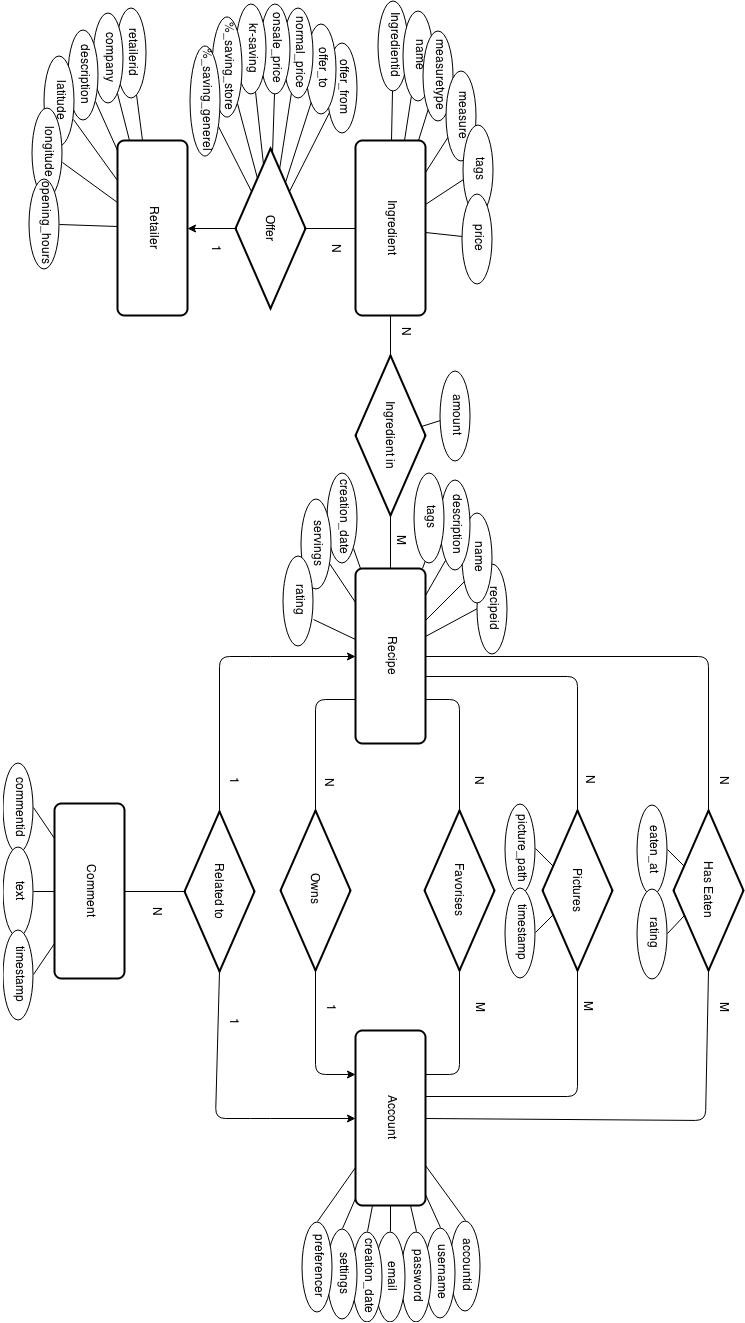
\includegraphics[width=0.9\textwidth]{Pictures/ERdiagram}
\caption{The final ER diagram of the database}
\end{figure}

A lot of these relations speak for themselves, and the entire amount of relationships between account and recipe rather intuitive. We have chosen not to gather all the data in a single relationship as we want perform quick queries on the database rather than save memory. This is one of the advantages of having a stationary server with a large amount of memory available, it is possible to focus solely on performance. 

The biggest table in terms of sheer numbers would be ingredientIn, as each recipe has a lot of different ingredients. This has been accommodated for by moving most attributes to either recipe or ingredient, and we make sure to query through IngredientIn before joining any of these together.

